\documentclass[letterpaper]{article}
\usepackage{amssymb}
\usepackage{amsmath,amsthm}
\usepackage{tikz}
\usepackage{tikz}
\usetikzlibrary{intersections}
\usepackage{tikz}
\usetikzlibrary{arrows.meta}
\usepgflibrary{decorations.markings}
\usetikzlibrary{through}
\usetikzlibrary{decorations.pathmorphing}
\usetikzlibrary{backgrounds}
\usetikzlibrary{decorations.pathreplacing}
\usetikzlibrary{calc}

\begin{document}

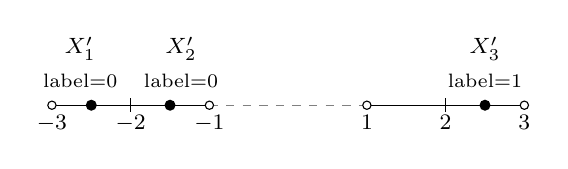
\begin{tikzpicture}
\coordinate [draw, label={below:\footnotesize{$-3$}}] (pm3) at (-3,0);
\coordinate [draw, label=below:\footnotesize{$-1$}] (pm1) at (-1,0);
\path[draw] (pm3) -- (pm1) coordinate[midway] (pm3Ppm1);

\coordinate [draw, label=below:\footnotesize{$3$}] (p3) at (3,0);
\coordinate [draw, label=below:\footnotesize{$1$}] (p1) at (1,0);
\path[draw] (p3) -- (p1) coordinate[midway] (p3Pp1);


\coordinate [draw, label=below:\footnotesize{$-2$}] (pm2) at (-2,0);
\coordinate [draw, label=below:\footnotesize{$2$}] (p2) at (2,0);

\path [draw, name path=qiPq1T]  ($(pm2)!2.5pt!270:(pm3)$) -- ($(pm2)!2.5pt!90:(pm3)$);
\path [draw, name path=qiPq1T]  ($(p2)!2.5pt!270:(p3)$) -- ($(p2)!2.5pt!90:(p3)$);

\path [name path = m1P1, color=gray, dashed, draw] (pm1) -- (p1) coordinate[midway] (m1P1);

\foreach \point in {pm1, pm3, p1, p3}
\draw [black, fill=white] (\point) circle (1.5pt);

\coordinate [draw, label={[align=center,yshift=3pt, xshift=-4pt]\footnotesize{$X'_1$}\\\scriptsize{label=$0$}}] (X1) at (-2.5,0);
\coordinate [draw, label={[align=center,yshift=3pt, xshift=4pt]\footnotesize{$X'_2$}\\\scriptsize{label=$0$}}] (X2) at (-1.5,0);
\coordinate [draw, label={[align=center,yshift=3pt]\footnotesize{$X'_3$}\\\scriptsize{label=$1$}}] (X3) at (2.5,0);

\foreach \point in {X1, X2, X3}
\fill [black] (\point) circle (2pt);

\end{tikzpicture}

\end{document}